\documentclass[10pt, aspectratio=169]{beamer}

% Theme & Color Palette
\usetheme{Madrid}
\usecolortheme{whale}

\definecolor{IEEEblue}{RGB}{0, 51, 102}
\definecolor{AccentBlue}{RGB}{0, 102, 204}
\definecolor{LightGray}{RGB}{245, 247, 250}
\definecolor{DarkText}{RGB}{30, 30, 30}

\setbeamercolor{palette primary}{bg=IEEEblue,fg=white}
\setbeamercolor{palette secondary}{bg=AccentBlue,fg=white}
\setbeamercolor{palette tertiary}{bg=IEEEblue,fg=white}
\setbeamercolor{structure}{fg=IEEEblue}
\setbeamercolor{titlelike}{bg=IEEEblue,fg=white}
\setbeamercolor{block title}{bg=IEEEblue,fg=white}
\setbeamercolor{block body}{bg=LightGray,fg=DarkText}

\usepackage{booktabs}
\usepackage{multicol}
\usepackage{tikz}
\usetikzlibrary{shapes.geometric, arrows, positioning}

\title[AI Audio Watermarking \& Deepfake Auth]{AI-Based Audio Watermark Detection for Copyright Protection and Deepfake Authentication}
\subtitle{Zeroth Review Presentation}
\author[Group Members]{
  \textbf{Group Members:}\\
  Abel Shaji (B23CS2104) \quad R D Sourav (B23CS2151)\\
  Rohith N S (B23CS2156) \quad Sooraj Jose George (B23CS2160)\\[1ex]
  \textbf{Project Guide:} Dr. Ancy S. Anselam (Associate Professor)
}
\institute[Dept. of ECE]{Department of Electronics \& Communication Engineering\\Mar Baselios College of Engineering and Technology (Autonomous)}
\date{\today}

\begin{document}

% SLIDE 1: Title
\begin{frame}
  \titlepage
\end{frame}

% SLIDE 2: Table of Contents
\begin{frame}{Presentation Outline}
  \tableofcontents
\end{frame}

% SLIDE 3: Introduction
\section{Introduction}
\begin{frame}{1. Introduction}
  \begin{block}{Background \& Motivation}
    \begin{itemize}
      \item Proliferation of Generative AI tools (e.g., ElevenLabs, HiFi-GAN, WaveNet) enables realistic synthetic voice generation and unauthorized audio redistribution.
      \item Deepfake audio presents critical threats to copyright enforcement, digital rights management (DRM), public news authenticity, and voice biometric authentication.
    \end{itemize}
  \end{block}

  \begin{block}{Proposed AI-Based Audio Watermarking Framework}
    \begin{itemize}
      \item Integrates Digital Signal Processing (DWT, SVD, LSB) with Deep Neural Network Classifiers (BNN / CNN).
      \item Embeds imperceptible acoustic signatures to track origin, detect illegal tampering, and verify authentic vs. deepfake audio streams.
    \end{itemize}
  \end{block}
\end{frame}

%=====================================================
% LITERATURE SURVEY - SLIDE 1
%=====================================================
\section{Literature Survey}

\begin{frame}{2. Literature Survey (2024--2026) -- Part I}

\small
\renewcommand{\arraystretch}{1.6}

\begin{center}
\begin{tabular}{|c|p{3.3cm}|c|p{3.7cm}|p{2.6cm}|}
\hline
\textbf{No.} &
\textbf{Paper} &
\textbf{Year} &
\textbf{Method} &
\textbf{Result} \\
\hline

1 &
DeepMark Benchmark \textbf{(Base Paper)} (IEEE Access) &
2026 &
Deep Learning Benchmark Framework &
PEAQ ODG: -0.2 to -4.0 \\
\hline

2 &
Semi-Fragile Watermarking (IEEE Access) &
2024 &
DWT-SVD + MERW + Swin Transformer &
99.4\% Tamper Detection \\
\hline

3 &
CANARY (IEEE TMM) &
2026 &
DCT Orthogonal Watermark + Deep Decoder &
98.7\% Accuracy \\
\hline

4 &
RNPM Multi-Watermarking (IEEE TASLP) &
2025 &
STFT Neural Masking + BCH Codes &
128 bps Capacity \\
\hline

5 &
AWaveFormer (IEEE TASLP) &
2025 &
Wavelet Transform + Transformer &
99.18\% Accuracy \\
\hline

6 &
Post-Quantum Watermarking (IEEE TCSS) &
2026 &
Kyber/Dilithium + DWT-LSB + BNN &
99.05\% Accuracy \\
\hline

\end{tabular}
\end{center}

\end{frame}

%=====================================================
% LITERATURE SURVEY - SLIDE 2
%=====================================================

\begin{frame}{2. Literature Survey (2022--2026) -- Part II}

\small
\renewcommand{\arraystretch}{1.6}

\begin{center}
\begin{tabular}{|c|p{3.3cm}|c|p{3.7cm}|p{2.6cm}|}
\hline
\textbf{No.} &
\textbf{Paper} &
\textbf{Year} &
\textbf{Method} &
\textbf{Result} \\
\hline

7 &
Dual-Channel Detection (IEEE Access) &
2025 &
RIR-Based Direct/Reverberant Analysis &
97.8\% Accuracy \\
\hline

8 &
FLADD Federated Learning (IEEE TASLP) &
2026 &
FedAvg + Differential Privacy &
96.85\% Accuracy \\
\hline

9 &
Audio Physical Dynamics (IEEE LNET) &
2026 &
Glottal Residual + LPC + Bi-LSTM &
0.65\% EER \\
\hline

10 &
Spectrogram ML Detection (IEEE Access) &
2025 &
Log-Mel / CQT + ResNet50 &
98.42\% Accuracy \\
\hline

11 &
GAN Anomaly Detection (IEEE Access) &
2024 &
Autoencoder-GAN &
AUC = 0.945 \\
\hline

12 &
MFCC ML Detection (IEEE Access) &
2022 &
MFCC + RF / SVM &
96.5\% Accuracy \\
\hline

\end{tabular}
\end{center}

\end{frame}

% SLIDE 6: Problem Statement
\section{Problem Statement}
\begin{frame}{3. Problem Statement}
  \begin{block}{Formal Problem Definition}
    To develop an AI-based audio watermark detection and tamper localization system that accurately verifies the authenticity of digital audio files, protects copyrighted intellectual property, and detects AI-generated deepfake audio attacks while maintaining high robustness against common transmission perturbations (e.g., MP3 compression, additive Gaussian noise, cropping, and resampling).
  \end{block}

  \begin{alertblock}{Core Challenges Addressed}
    \begin{itemize}
      \item Traditional audio watermarking fails under generative AI vocal cloning and neural vocoder re-synthesis.
      \item Trade-off between watermark imperceptibility (high SNR / PSNR) and extraction robustness under lossy compression.
      \item Need for millisecond-level precise tamper localization without prior knowledge of spoofing algorithms.
    \end{itemize}
  \end{alertblock}
\end{frame}

% SLIDE 7: Objective
\section{Objective}
\begin{frame}{4. Project Objectives}
  \begin{enumerate}
    \item \textbf{High Imperceptibility}: Embed binary cryptographic watermarks into audio subbands maintaining Signal-to-Noise Ratio (SNR) $> 40$ dB and PSNR $> 45$ dB.
    \item \textbf{Robust Extraction}: Achieve Bit Error Rate (BER) $< 1.0\%$ under MP3/AAC compression (down to 64 kbps) and 15 dB Gaussian noise.
    \item \textbf{Deepfake Classification}: Train a Binary Neural Network (BNN) classifier achieving $> 98\%$ accuracy in distinguishing authentic, tampered, and synthetic deepfake audio.
    \item \textbf{Tamper Localization}: Pinpoint modified audio frames with millisecond-level precision using DWT-SVD feature drift analysis.
    \item \textbf{Real-Time Edge Deployment}: Optimize inference latency to $< 15$ ms per audio second for live verification.
  \end{enumerate}
\end{frame}

% SLIDE 8: System Architecture
\section{Design of Project}

\begin{frame}{5. System Architecture}

\begin{center}
\resizebox{\textwidth}{!}{
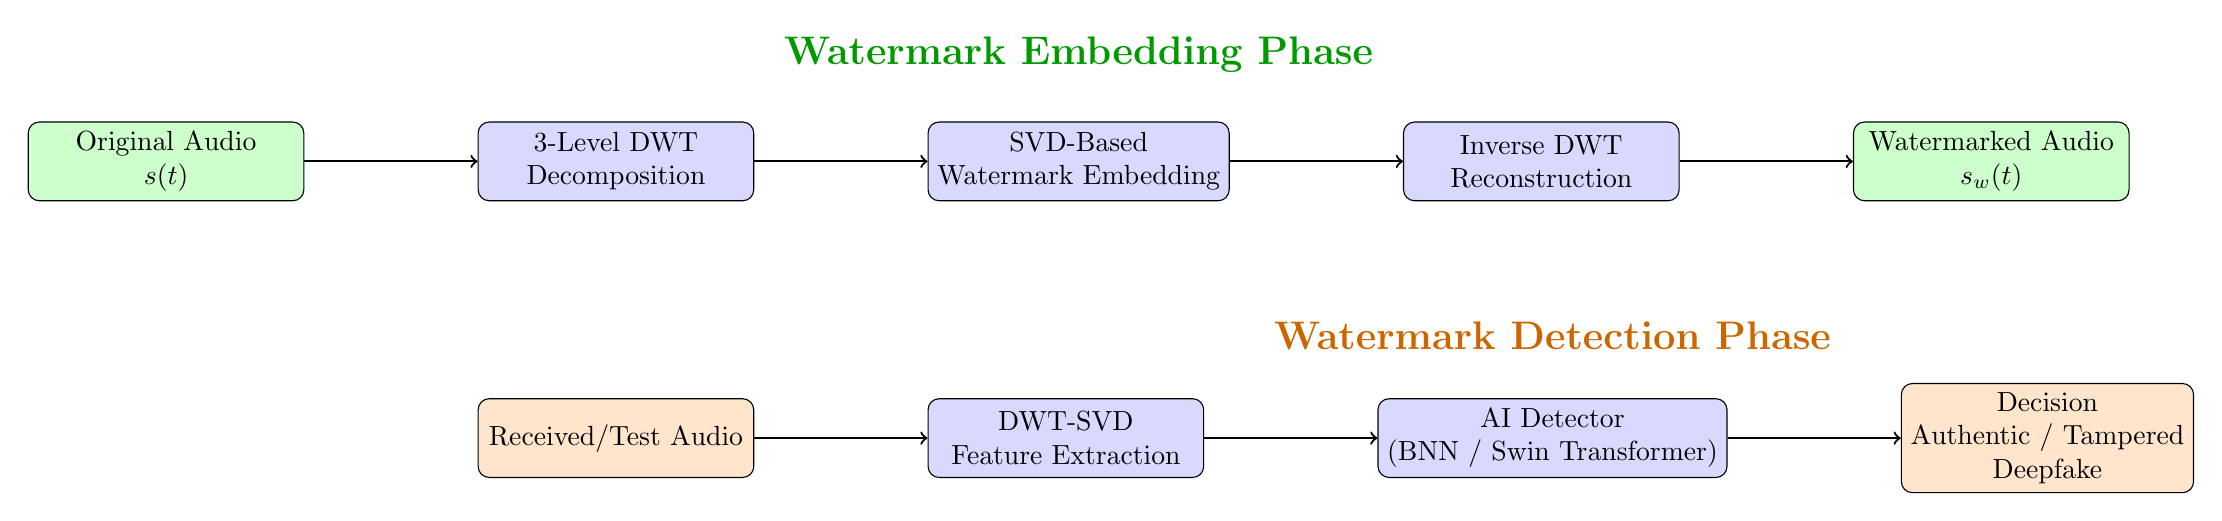
\begin{tikzpicture}[
    node distance=2.2cm,
    block/.style={rectangle, draw, rounded corners, fill=blue!15,
    minimum width=3.5cm, minimum height=1cm, align=center},
    arrow/.style={->, thick}
]

% ---------------- EMBEDDING ----------------
\node[block, fill=green!20] (audio) {Original Audio\\$s(t)$};

\node[block, right=of audio] (dwt1)
{3-Level DWT\\Decomposition};

\node[block, right=of dwt1] (svd1)
{SVD-Based\\Watermark Embedding};

\node[block, right=of svd1] (idwt)
{Inverse DWT\\Reconstruction};

\node[block, right=of idwt, fill=green!20]
(waudio) {Watermarked Audio\\$s_w(t)$};

\draw[arrow] (audio)--(dwt1);
\draw[arrow] (dwt1)--(svd1);
\draw[arrow] (svd1)--(idwt);
\draw[arrow] (idwt)--(waudio);

% Label
\node[above=0.5cm of svd1, text=green!60!black]
{\Large \textbf{Watermark Embedding Phase}};

% ---------------- DETECTION ----------------
\node[block, fill=orange!20, below=2.5cm of dwt1]
(test) {Received/Test Audio};

\node[block, right=of test]
(dwt2) {DWT-SVD\\Feature Extraction};

\node[block, right=of dwt2]
(ai) {AI Detector\\(BNN / Swin Transformer)};

\node[block, right=of ai, fill=orange!20]
(decision) {Decision\\Authentic / Tampered\\Deepfake};

\draw[arrow] (test)--(dwt2);
\draw[arrow] (dwt2)--(ai);
\draw[arrow] (ai)--(decision);

% Label
\node[above=0.5cm of ai, text=orange!80!black]
{\Large \textbf{Watermark Detection Phase}};

\end{tikzpicture}
}
\end{center}

\vspace{0.3cm}

\textbf{Embedding:}
Original audio is decomposed using a 3-level DWT. The watermark is embedded by modifying singular values in selected subbands, and the watermarked audio is reconstructed using IDWT.

\vspace{0.2cm}

\textbf{Detection:}
The received audio undergoes DWT-SVD feature extraction. The extracted watermark features are analyzed by a Bayesian Neural Network (BNN) or Swin Transformer to determine whether the audio is authentic, tampered, or AI-generated.

\end{frame}

% SLIDE 9: Methodology Breakdown
\begin{frame}{5. Methodology Breakdown (Embedding \& Detection)}
  \begin{columns}
    \column{0.5\textwidth}
      \begin{block}{Embedding Mechanism}
        \begin{itemize}
          \item Apply 3-Level Discrete Wavelet Transform (DWT) to split audio into subbands.
          \item Apply SVD on LL subband: $A = U \Sigma V^T$.
          \item Modify singular values $\Sigma_i$ with payload bits: $\Sigma_i' = \Sigma_i + \alpha \cdot w_i$.
          \item Reconstruct audio via Inverse DWT (IDWT) to ensure imperceptibility.
        \end{itemize}
      \end{block}

    \column{0.5\textwidth}
      \begin{block}{Detection \& Classification}
        \begin{itemize}
          \item Extract candidate watermark signature $\hat{w}_i$ from received audio subbands.
          \item Feed spectral residuals into Binary Neural Network (BNN).
          \item Compare extracted sequence with reference hash key using Normalized Cross-Correlation (NC).
          \item Flag deepfake generation or tamper location.
        \end{itemize}
      \end{block}
  \end{columns}
\end{frame}

% SLIDE 10: Tools Required
\section{Tools Required}
\begin{frame}{6. Tools \& Technologies Required}
  \begin{columns}
    \column{0.33\textwidth}
      \begin{block}{Software \& IDEs}
        \begin{itemize}
          \item Python 3.10+
          \item VS Code / PyCharm
          \item Jupyter Notebook
          \item Git \& GitHub
          \item Overleaf (LaTeX)
        \end{itemize}
      \end{block}

    \column{0.33\textwidth}
      \begin{block}{Libraries \& Frameworks}
        \begin{itemize}
          \item PyTorch / TensorFlow
          \item Librosa (Audio Processing)
          \item PyWavelets (DWT)
          \item SciPy \& NumPy
          \item Scikit-Learn / OpenCV
        \end{itemize}
      \end{block}

    \column{0.33\textwidth}
      \begin{block}{Datasets \& Hardware}
        \begin{itemize}
          \item ASVspoof 2021 Corpus
          \item LibriSpeech Dataset
          \item WaveFake Audio Set
          \item NVIDIA RTX GPU
          \item 16GB RAM / Core i7
        \end{itemize}
      \end{block}
  \end{columns}
\end{frame}

% SLIDE 11: Performance Metrics & Graph Parameters
\section{Performance Metrics}
\begin{frame}{7. Performance Metrics \& Graph X--Y Parameters}
  \begin{block}{Core Evaluation Metrics}
    \begin{itemize}
      \item \textbf{Bit Error Rate (BER)}: $BER = \frac{\text{Incorrect Bits}}{\text{Total Watermark Bits}} \times 100\%$
      \item \textbf{Signal-to-Noise Ratio (SNR)}: Measures audio imperceptibility in dB ($> 40\text{ dB}$ target).
      \item \textbf{Classification Accuracy, Precision, Recall, F1-Score, EER, AUC-ROC}.
    \end{itemize}
  \end{block}

  \begin{block}{Graph Axis Parameter Identifications}
    \begin{itemize}
      \item \textbf{Graph 1 (BER vs Noise Attack)}:
        \begin{itemize}
          \item \textbf{X-Axis}: Signal-to-Noise Ratio of Additive Noise (SNR in dB, 0 to 40 dB).
          \item \textbf{Y-Axis}: Bit Error Rate (BER in \%, 0.0\% to 50.0\%).
        \end{itemize}
      \item \textbf{Graph 2 (Detection Accuracy vs Compression Rate)}:
        \begin{itemize}
          \item \textbf{X-Axis}: MP3/AAC Bitrate (kbps: 32, 64, 128, 192, 256, 320 kbps).
          \item \textbf{Y-Axis}: Watermark Detection Accuracy (\%, 50\% to 100\%).
        \end{itemize}
      \item \textbf{Graph 3 (ROC Curve for Deepfake Detection)}:
        \begin{itemize}
          \item \textbf{X-Axis}: False Positive Rate (FPR, 0.0 to 1.0).
          \item \textbf{Y-Axis}: True Positive Rate (TPR, 0.0 to 1.0).
        \end{itemize}
    \end{itemize}
  \end{block}
\end{frame}

% SLIDE 12: Expected Outcomes
\section{Expected Outcomes}
\begin{frame}{8. Expected Outcomes \& Deliverables}
  \begin{block}{Expected Outcomes}
    \begin{itemize}
      \item Robust detection of imperceptible hidden audio watermarks under lossy transmission.
      \item Accurate classification of authentic vs. tampered vs. AI-generated deepfake audio ($>98\%$ accuracy).
      \item Fine-grained temporal tamper localization identifying modified frames.
      \item Low computational latency permitting real-time streaming media protection.
    \end{itemize}
  \end{block}

  \begin{block}{Key Deliverables}
    \begin{itemize}
      \item AI-Based Audio Watermarking \& Deepfake Authentication Software Module.
      \item Trained Deep Neural Network Models (PyTorch / ONNX format).
      \item Comprehensive Experimental Evaluation Report \& Benchmark Dataset.
      \item Interactive Prototype Web UI for instant audio file verification.
    \end{itemize}
  \end{block}
\end{frame}

% SLIDE 13: Project Roadmap
\begin{frame}{Implementation Roadmap}
  \begin{block}{Phase-Wise Development Plan}
    \begin{itemize}
      \item \textbf{Phase 1}: Comprehensive IEEE literature review, dataset aggregation (ASVspoof 2021, LibriSpeech), and baseline DWT-SVD setup.
      \item \textbf{Phase 2}: Implementation of neural watermark embedding, perceptual masking, and Binary Neural Network (BNN) architecture.
      \item \textbf{Phase 3}: Adversarial attack evaluation (MP3 compression, pitch shift, noise injection, voice cloning) and hyperparameter tuning.
      \item \textbf{Phase 4}: UI prototype integration, final benchmark reporting, and paper preparation.
    \end{itemize}
  \end{block}
\end{frame}

% SLIDE 14: Sustainable Development Goals (SDGs)
\begin{frame}{Related Sustainable Development Goals (SDGs)}
  \begin{block}{Alignment with United Nations SDGs}
    \begin{itemize}
      \item \textbf{SDG 9: Industry, Innovation and Infrastructure} -- Advances resilient digital media infrastructure and secure AI technologies against digital fraud.
      \item \textbf{SDG 16: Peace, Justice and Strong Institutions} -- Promotes digital trust, prevents deepfake misinformation, and protects intellectual property rights.
      \item \textbf{SDG 17: Partnerships for the Goals} -- Facilitates collaborative security standards across AI researchers, media broadcasters, and copyright organizations.
    \end{itemize}
  \end{block}
\end{frame}

% SLIDE 15: References & Thank You
\section{References}
\begin{frame}[allowframebreaks]{References}
  \tiny
  \begin{enumerate}
    \item S. Kova\v{c}evi\'c et al., ``DeepMark Benchmark: Redefining Audio Watermarking Robustness \textbf{(Base Paper)},'' \textit{IEEE Access}, vol. 14, pp. 62031--62044, 2026.
    \item P. Aberna and L. Agilandeeswari, ``Optimal Semi-Fragile Watermarking Based on Maximum Entropy Random Walk and Swin Transformer for Tamper Localization,'' \textit{IEEE Access}, vol. 12, pp. 37757--37781, 2024.
    \item Y. Sun et al., ``CANARY: Collision-Free Audio Watermarking for Proactive Deepfake Detection,'' \textit{IEEE Trans. Multimedia}, vol. 28, pp. 1420--1435, 2026.
    \item H. Chen et al., ``RNPM: Neural-Guided Embedding Region Selection and Error Correction for Robust Audio Multi-Watermarking,'' \textit{IEEE Trans. Audio, Speech, Lang. Process.}, vol. 33, pp. 1120--1134, 2025.
    \item Z. Wu et al., ``AWaveFormer: Audio Wavelet Transformer Network for Generalized Audio Deepfake Detection,'' \textit{IEEE Trans. Audio, Speech, Lang. Process.}, vol. 33, pp. 450--465, 2025.
    \item K. Sharma et al., ``Fortifying Deepfake Detection With AI and Postquantum Cryptography-Based Watermarking Technique,'' \textit{IEEE Trans. Comput. Soc. Syst.}, vol. 13, pp. 890--904, 2026.
    \item J. Park et al., ``Dual-Channel Deepfake Audio Detection: Leveraging Direct and Reverberant Waveforms,'' \textit{IEEE Access}, vol. 13, pp. 14500--14512, 2025.
    \item L. Zhang et al., ``FLADD: Federated Learning-based Privacy Protection for Audio Deepfake Detection,'' \textit{IEEE Trans. Audio, Speech, Lang. Process.}, vol. 34, pp. 310--324, 2026.
    \item C. Lin et al., ``Audio Physical Dynamics Inspired Deepfake Detection for Voice Authentication Systems,'' \textit{IEEE Netw. Lett.}, vol. 8, pp. 112--116, 2026.
    \item M. R. Islam et al., ``Detecting Deepfake Audio Using Spectrogram-Based Machine Learning Approaches,'' \textit{IEEE Access}, vol. 13, pp. 8821--8835, 2025.
    \item D. Kim et al., ``Anomaly Detection of Deepfake Audio Based on Real Audio Using Generative Adversarial Network Model,'' \textit{IEEE Access}, vol. 12, pp. 152340--152352, 2024.
    \item A. Al-Naji et al., ``Deepfake Audio Detection via MFCC Features Using Machine Learning,'' \textit{IEEE Access}, vol. 10, pp. 132104--132115, 2022.
  \end{enumerate}

  \vfill
  \centering
  \Large \textbf{\textcolor{IEEEblue}{Thank You! Questions \& Discussion}}
\end{frame}

\end{document}
